\documentclass[a4paper,12pt]{article}
\usepackage[utf8]{inputenc}
\usepackage{graphicx}
\usepackage{hyperref}
\usepackage{natbib}
\usepackage{url}
\usepackage{tabularx}
\usepackage{booktabs}

\title{Computational Mathematics for AI: Numerical Methods and Distributed Computing for Deep Learning on Big Data}
\author{Pouya Ataei}
\date{\today}

\begin{document}

\maketitle

\section{Introduction}
This document outlines the protocol for a systematic literature review (SLR) on computational mathematics for AI, focusing on numerical methods and distributed computing techniques for deep learning on big data. The review will follow the PRISMA guidelines \citep{moher2009preferred} and Kitchenham's methodology for SLRs in software engineering \citep{kitchenham2007guidelines}.

\section{Background}
\subsection{Rationale}
%As deep learning models grow in complexity and data volumes continue to increase, there is a critical need to understand and optimize the computational methods underpinning these systems.


Deep learning has emerged as a transformative technology, providing state-of-the-art solutions for a wide range of big data applications. 
However, as the complexity of these models grows and data volumes continue to increase, there is a significant need to understand and optimize the computational methods underpinning these systems.
 Numerical methods and distributed computing play pivotal roles in addressing the computational challenges associated with training and deploying deep learning models on large-scale datasets.
Recent advancements in this field have led to various approaches for optimizing performance, scalability, and resource efficiency.

One of the key challenges in deep learning is efficiently handling the vast amounts of data and computational requirements involved in training deep learning models. 
Numerical methods such as optimization algorithms are fundamental for training these models, particularly in ensuring convergence and minimizing loss functions effectively.
 As highlighted by~\cite{najafabadi2015deep}, the integration of deep learning techniques with big data analytics presents numerous challenges, particularly in terms of computational efficiency and scalability. This necessitates a deeper exploration of computational mathematics to improve model training and inference.

In addition to numerical methods, distributed computing techniques have become increasingly crucial in the context of big data and deep learning.\cite{yan2023computational} 
outlines the theoretical foundations and practical implementations of computational methods for deep learning, emphasizing the importance of distributed frameworks. 
Techniques such as GPU acceleration, federated learning, and parallel processing are instrumental in scaling deep learning models to meet the demands of large-scale data processing \cite{dehghani2023distributed}. 
These distributed computing approaches enable more efficient training by distributing workloads across multiple nodes or devices, thus reducing training time and improving scalability.

Overall, the intersection of numerical methods and distributed computing forms the backbone of scalable deep learning systems for big data applications. 
By synthesizing knowledge from both domains, it is possible to create more efficient deep learning models capable of processing large datasets with reduced computational overhead.


This review aims to synthesize current knowledge on numerical methods and distributed computing techniques specifically applied to deep learning in big data contexts.

\subsection{Objectives}
The primary objectives of this SLR are:
\begin{enumerate}
    \item To identify and categorize state-of-the-art numerical methods used in deep learning for big data.
    \item To evaluate the effectiveness of various distributed computing techniques for scaling deep learning to big data problems.
    \item To compare these methods and techniques in terms of computational efficiency, scalability, and accuracy.
    \item To identify emerging trends and future directions in this field.
\end{enumerate}
\section{Related work}

A considerable amount of research has focused on enhancing deep learning's computational efficiency and scalability, particularly through advancements in numerical methods and distributed computing. 
The work by~\cite{najafabadi2015deep} provides an extensive overview of deep learning applications in big data analytics, emphasizing the inherent challenges in managing large-scale data 
and the computational power required. The authors discuss various deep learning architectures and the specific numerical methods used to optimize these models, setting a foundation for understanding 
the computational needs of big data-driven deep learning.

The book by~\cite{yan2023computational} presents a comprehensive discussion on the computational methods for deep learning, detailing the theoretical aspects of optimization algorithms and their implementation in practical scenarios. This work bridges the gap between theory and practical deployment, offering insights into the challenges of implementing these methods in a distributed environment. The book highlights the importance of selecting appropriate numerical methods to ensure both convergence and computational efficiency.

A survey by~\cite{zhang2023distributed} delves into distributed deep learning frameworks, discussing the evolution from traditional distributed machine learning to more sophisticated distributed deep learning systems. It explores various distributed computing techniques such as federated learning, GPU acceleration, and parallel processing, which are essential for scaling deep learning models for big data applications. The survey compares different distributed frameworks, analyzing their scalability, efficiency, and suitability for diverse deep learning tasks.

Similarly,~\cite{li2019federated} provides a foundational overview of federated learning, a decentralized approach to training models without sharing raw data between nodes. This technique is especially useful for privacy-sensitive applications in big data. The authors discuss federated learning’s architecture, key challenges, and promising results in scaling deep learning for real-world applications.

\cite{li2020survey} offers a detailed survey of scalable deep learning techniques, specifically focusing on efficient parallel processing and distributed systems. The work discusses both hardware-based approaches, such as GPU acceleration, and software-based frameworks like Apache Spark, which have shown promise in reducing the computational time required for large-scale models, making deep learning more feasible for real-time applications.

Further,~\cite{ben2019demystifying} provides insights into optimization methods specifically tailored for big data in deep learning. The authors review key numerical methods and optimization algorithms, addressing their impact on model convergence and performance. This paper is particularly valuable for understanding the trade-offs between computational cost and accuracy, which are central to deep learning in big data contexts.

Overall, the related work in this domain underscores the interplay between numerical optimization techniques and distributed computing as fundamental enablers of scalable deep learning. These works collectively highlight the importance of computational efficiency, scalability, and the need for continued research to address the complexities of big data-driven deep learning.




\section{Research Methodology}

This study employs a comprehensive approach combining two systematic literature reviews (SLRs) with subsequent meta-analysis and network analysis. The methodology is structured into seven distinct phases:

\subsection{Phase 1: Planning and Protocol Development}

\subsubsection{Research Questions}
For SLR 1 (Numerical Methods):
\begin{enumerate}
    \item[RQ1.1] What are the state-of-the-art numerical methods used in deep learning for big data?
    \item[RQ1.2] How do these methods perform in terms of computational efficiency and accuracy?
\end{enumerate}

For SLR 2 (Distributed Computing Techniques):
\begin{enumerate}
    \item[RQ2.1] What distributed computing techniques are used for scaling deep learning to big data problems?
    \item[RQ2.2] How effective are these techniques in terms of scalability and performance?
\end{enumerate}

\subsubsection{Literature Review Classification Framework}
We will use Cooper's taxonomy \citep{cooper1988} to classify the literature in both SLRs:

\begin{table}[h]
\caption{Adaptation of Cooper's Literature Review Taxonomy}
\begin{tabularx}{\textwidth}{lX}
\toprule
Characteristic & Categories \\
\midrule
(a) Focus     & Research outcomes, Research methods, Theories, Practices or applications \\
(b) Goal      & Integration, Criticism, Identification of central issues \\
(c) Perspective & Neutral representation, Espousal of position \\
(d) Coverage  & Exhaustive, Exhaustive with selective citation, Representative, Central or pivotal \\
(e) Organization & Historical, Conceptual, Methodological \\
(f) Audience  & Specialized scholars, General scholars, Practitioners or policymakers, General public \\
\bottomrule
\end{tabularx}
\end{table}

This classification will be applied to each included study during the data extraction phase. It will help us to:

\begin{itemize}
    \item Systematically categorize the nature and scope of each study
    \item Identify patterns and trends in the literature
    \item Ensure a balanced representation of different types of research in our review
    \item Tailor our findings to different audience needs
    \item Guide our analysis and synthesis of the literature
\end{itemize}

The classification results will be used in Phase 6 (Study Classification and Bias Assessment) to provide additional context for interpreting our findings and identifying gaps in the current research landscape.

\subsubsection{Search Strategy Development}
PICO-based search strings for each SLR:

SLR 1 (TITLE AND ABSTRACT SEARCH) :
\begin{verbatim}
("deep learning"
AND 
("numerical method*" 
OR "computational mathematics" 
OR "optimization algorithm*")
AND 
("big data"))
\end{verbatim}


\emph{IEEE Explore Search String:}

(("deep learning" AND ("numerical method*" OR "computational mathematics" OR "optimization algorithm*") AND ("big data")))

\emph{Scopus Search String:}

( TITLE-ABS ( "deep learning" ) AND ( TITLE-ABS ( "numerical method*" OR "computational mathematics" OR "optimization algorithm*" ) ) AND TITLE-ABS ( "big data" ) )

\emph{Aisel Search String:}
([[Title:"deep learning"] AND [Title: "numerical method*"]] OR [Title: "computational mathematics"] OR [[Title: "optimization algorithm*"] AND [Title: "big data"])

\emph{ACM Search String:}
([[[Title: "deep learning"] AND [Title: "numerical method*"]] OR [Title: "computational mathematics"] OR [[Title: "optimization algorithm*"] AND [Title: "big data"]]] AND [[Abstract: "deep learning"] OR [Abstract: "numerical method*"] OR [Abstract: "computational mathematics"] OR [Abstract: "optimization algorithm*"] OR [Abstract: "big data"]])
\emph{Springer Search String:}
( TITLE-ABS ( "deep learning" ) AND ( TITLE-ABS ( "numerical method*" OR "computational mathematics" OR "optimization algorithm*" ) ) AND TITLE-ABS ( "big data" ) )

\vline

SLR 2:
\begin{verbatim}
(("deep learning" OR "neural network*") AND 
("distributed computing" OR "parallel processing" OR 
"GPU acceleration" OR "federated learning") AND 
("big data" OR "large-scale") AND 
(scalability OR performance))
\end{verbatim}

\subsubsection{Information Sources}
IEEE Xplore, ACM Digital Library, SpringerLink, Scopus, Web of Science, JSTOR, AIS 

\subsubsection{Eligibility Criteria}
Inclusion criteria for SLR 1:
\begin{itemize}
    \item Studies published between January 1, 2014 and September 21, 2024
    \item Peer-reviewed journal articles and full conference papers
    \item English language publications
    \item Studies focusing on numerical methods for deep learning in big data contexts
    \item Research explicitly addressing computational efficiency or accuracy of numerical methods
    \item Studies providing quantitative, qualitative results or comparative analyses of numerical methods
\end{itemize}

Exclusion criteria for SLR 1:
\begin{itemize}
    \item Studies not explicitly addressing big data characteristics
    \item Publications without clear details on the numerical methods used
    \item Review papers, editorials, or opinion pieces
    \item Short papers (less than 10 pages), extended abstracts, or posters
    \item Duplicate studies or multiple publications of the same research
\end{itemize}
\subsection{Phase 2: Literature Search and Study Selection}

\subsubsection{Search Execution}

\begin{enumerate}
    \item Execute search strategy on selected databases
    \item Import results to a unified CSV file
\end{enumerate}

\subsubsection{Deduplication}

\begin{enumerate}
\item Remove duplicates

\end{enumerate}

\subsubsection{Initial Screening}

\begin{enumerate}
    \item Initial screening of titles and abstracts
    \item Following low inter-rater reliability (Krippendorff's a = 0.4), implemented Modified Delphi Protocol based on RAND/UCLA methodology \citep{fitch2001rand} and Dalkey's classical Delphi framework \citep{dalkey1969delphi}:
    
    \paragraph{Round 1: Anonymous Individual Assessment}
    \begin{itemize}
        \item Each reviewer independently screens 50 randomly selected papers
        \item Reviewers document detailed rationale for inclusion/exclusion decisions
        \item Responses collected via standardized electronic form
        \item Statistical analysis of agreement levels using methods described by \citet{diamond2014results}
    \end{itemize}
    
    \paragraph{Round 2: Controlled Feedback}
    \begin{itemize}
        \item Anonymous compilation of Round 1 decisions and rationales
        \item Distribution of statistical summary showing group response
        \item Identification of areas of agreement and disagreement
        \item Written feedback from each reviewer on points of disagreement
    \end{itemize}
    
    \paragraph{Round 3: Consensus Development}
    \begin{itemize}
        \item Structured meeting following nominal group technique \citep{delbecq1975group}
        \item Development of explicit screening criteria
        \item Documentation of specific examples for each criterion
        \item Creation of decision flowchart for ambiguous cases
    \end{itemize}



    \paragraph{Consensus Results}

\subsection{Methodological Background}
Following the Delphi-based consensus methodology outlined by \cite{dalkey1963experimental} and the systematic review guidelines of \cite{kitchenham2004procedures}, we conducted a structured consensus meeting to establish classification criteria. The meeting employed the Nominal Group Technique as described by \cite{delbecq1971group}, resulting in a formalized decision framework.

\subsection{Decision Framework Overview}
The consensus process established a hierarchical decision framework for paper classification, illustrated in Figure \ref{fig:decision-flow}. The framework implements a stage-gate approach with sequential evaluation criteria.

\begin{figure}
\centering
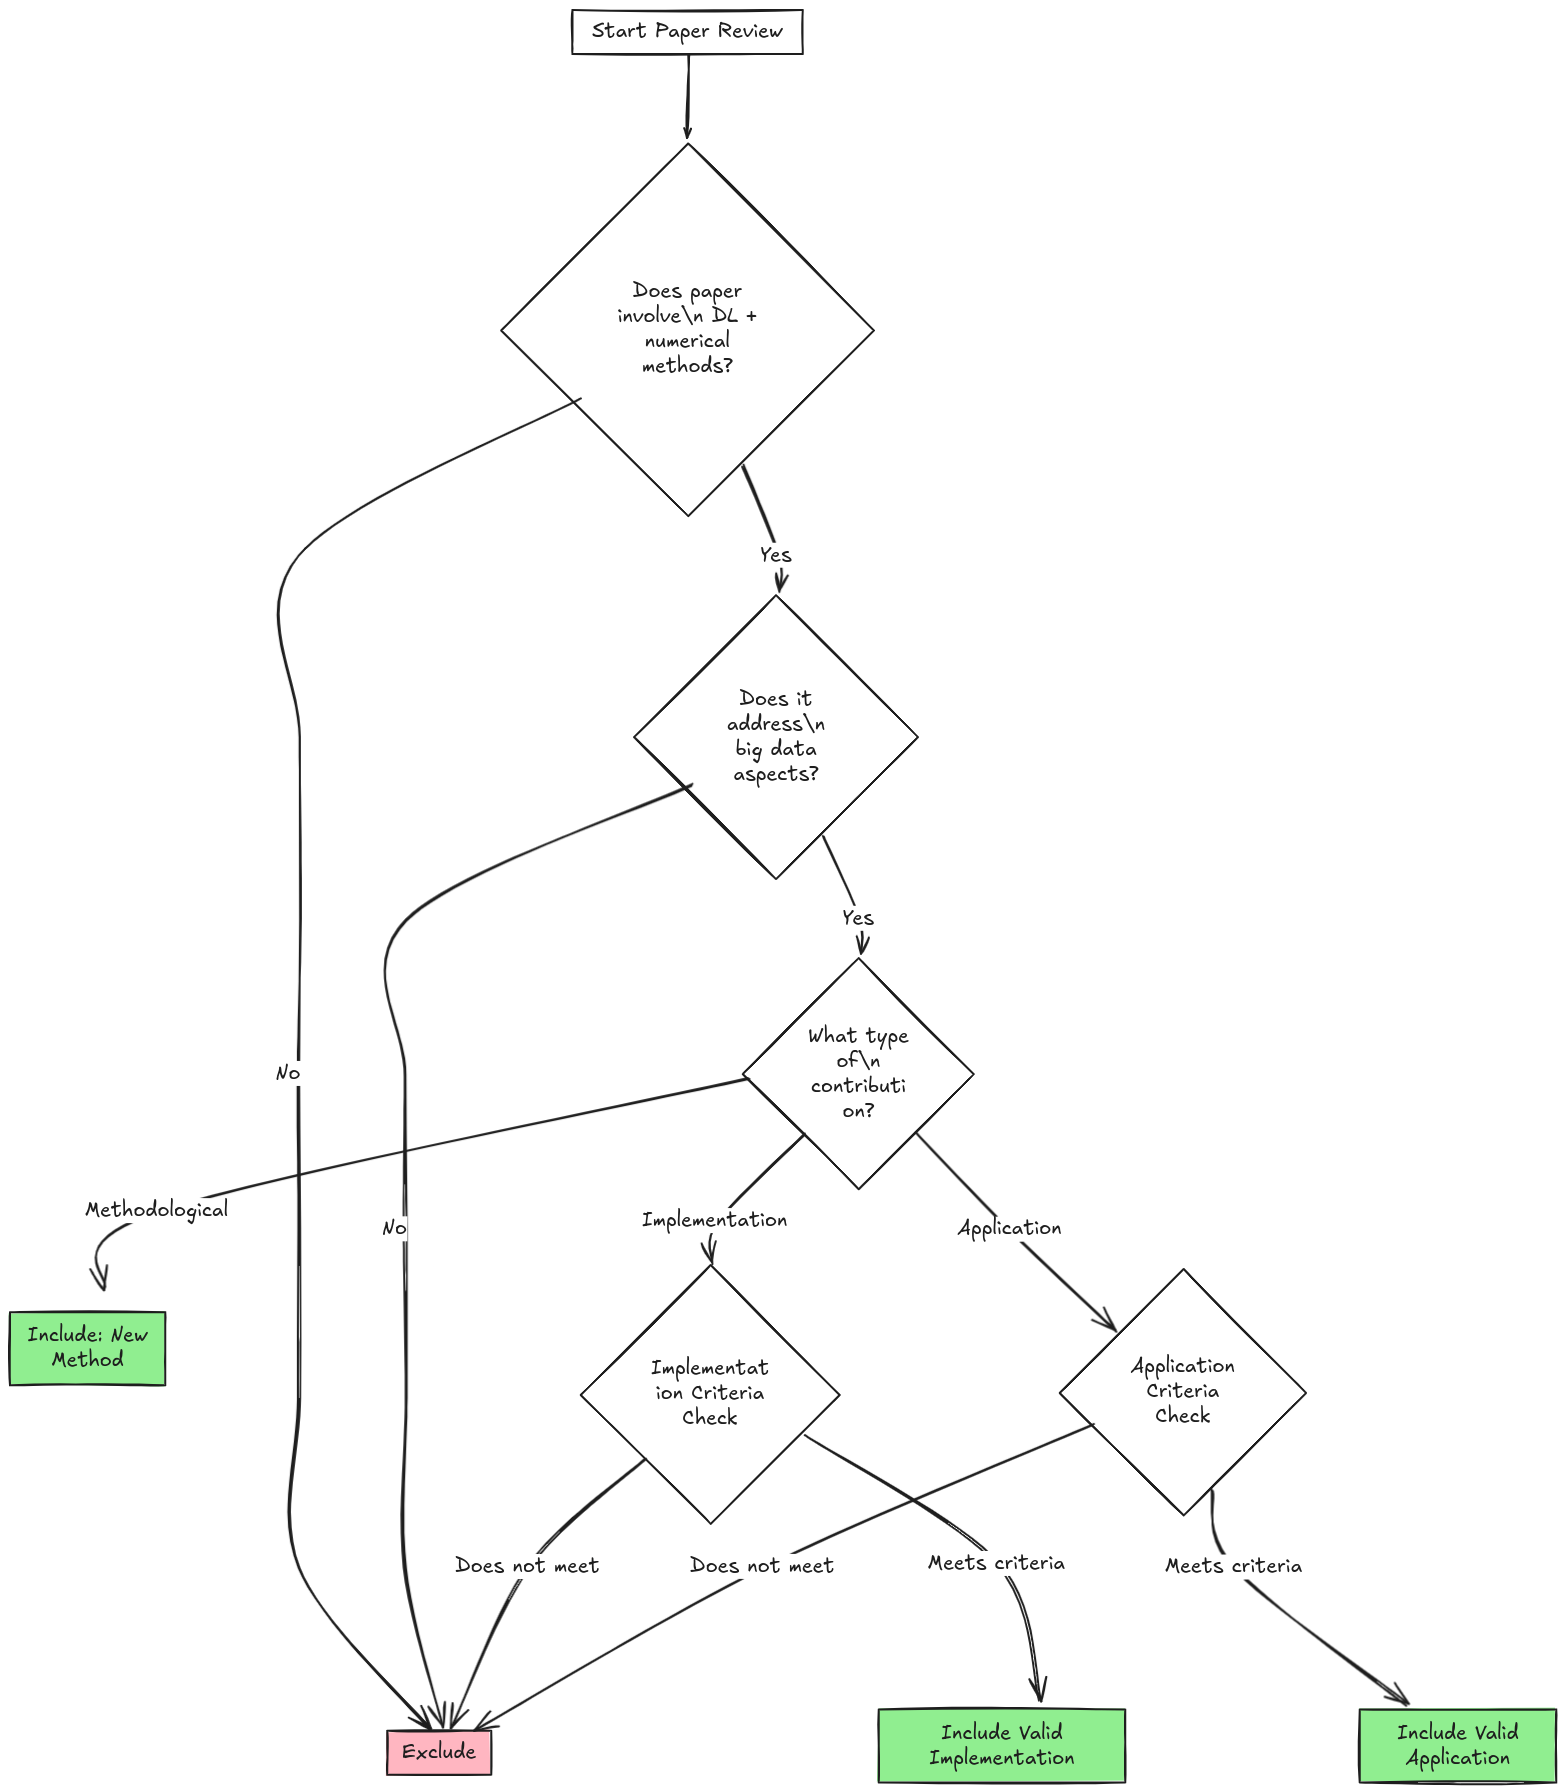
\includegraphics[width=15cm] {media/Company Structure.png}
\caption{Paper Classification Decision Framework}
\label{fig:decision-flow}
\end{figure}

\subsection{Primary Decision Gates}
Based on consensus deliberation, the following sequential decision gates were established:

\begin{enumerate}
    \item \textbf{Deep Learning and Numerical Methods Verification}
    \begin{itemize}
        \item Explicit use of deep learning techniques
        \item Clear numerical methods component
        \item Verifiable technical implementation or application
    \end{itemize}
    
    \item \textbf{Big Data Aspects Evaluation}
    \begin{itemize}
        \item Volume: Significant data scale as defined by \cite{laney2001data}
        \item Velocity: Real-time or streaming data considerations
        \item Variety: Heterogeneous data types
        \item Processing: Computational complexity requirements
    \end{itemize}
    
    \item \textbf{Contribution Type Classification}
    \begin{itemize}
        \item Implementation focus: Technical deployment emphasis
        \item Application focus: Domain adaptation emphasis
        \item Hybrid approaches: Primary contribution determination
    \end{itemize}
\end{enumerate}

[Previous Implementation and Application Criteria sections remain unchanged]

\subsection{Consensus-Based Classification Process}
The consensus meeting established the following process requirements:

\subsubsection{Initial Screening}
\begin{itemize}
    \item Independent evaluation of papers
    \item Application of primary decision gates
    \item Documentation of decision rationale
\end{itemize}

\subsubsection{Detailed Evaluation}
Papers passing initial screening undergo detailed evaluation against either:
\begin{itemize}
    \item Implementation criteria (minimum 2 of 3 required)
    \item Application criteria (minimum 2 of 3 required)
\end{itemize}

\subsubsection{Border Case Resolution}
The consensus established specific protocols for border cases:

\begin{enumerate}
    \item \textbf{Hybrid Contributions}
    \begin{itemize}
        \item Evaluate against both criteria sets
        \item Classify based on primary contribution
        \item Document dual-nature considerations
    \end{itemize}
    
    \item \textbf{Ambiguous Cases}
    \begin{itemize}
        \item Require third reviewer evaluation
        \item Apply decision framework strictly
        \item Document specific points of ambiguity
    \end{itemize}
    
    \item \textbf{Novel Approaches}
    \begin{itemize}
        \item Evaluate against established criteria
        \item Consider potential framework adaptation
        \item Document precedent-setting decisions
    \end{itemize}
\end{enumerate}

\subsection{Inter-Rater Reliability Requirements}
Based on \cite{krippendorff2004reliability}, the following reliability thresholds were established:

\begin{itemize}
    \item Initial screening: Krippendorff's a > 0.8
    \item Detailed evaluation: 85\% agreement minimum
    \item Border cases: Unanimous consensus required
\end{itemize}

\subsection{Framework Validation}
The classification framework was validated through:

\begin{enumerate}
    \item \textbf{Pilot Testing}
    \begin{itemize}
        \item Application to 50 sample papers
        \item Inter-rater reliability assessment
        \item Process refinement based on results
    \end{itemize}
    
    \item \textbf{Expert Review}
    \begin{itemize}
        \item Independent expert evaluation
        \item Framework refinement feedback
        \item Documentation of edge cases
    \end{itemize}
    
    \item \textbf{Statistical Validation}
    \begin{itemize}
        \item Agreement rate analysis
        \item Decision consistency evaluation
        \item Process efficiency metrics
    \end{itemize}
\end{enumerate}




    
    \paragraph{Round 4: Validation}
    \begin{itemize}
        \item Re-screening of original 50 papers using new criteria
        \item Calculation of new inter-rater reliability
        \item If Krippendorff's a > 0.8, proceed to full screening
        \item If a < 0.8, repeat Round 3 with focused discussion on remaining issues
    \end{itemize}
\end{enumerate}

\subsubsection{Deeper Screening}

\begin{enumerate}
    \item Full-text assessment of potentially eligible studies
\end{enumerate}


Document selection process should be done using PRISMA flow diagram.



\subsection{Phase 3: Quality Assessment}
The quality of individual studies will be assessed using a criteria made up of 7 elements, inspired by the CASP checklist for assessing qualitative research and Kitchenham's guidelines on empirical research in software engineering . This assessment will be applied to studies in both SLRs.

\subsubsection{Quality Assessment Criteria}
The criteria test literature on 4 major areas:

\paragraph{1. Minimum quality threshold:}
\begin{itemize}
    \item Does the study report empirical research or is it merely a 'lesson learnt' report based on expert opinion?
    \item Are the objectives and aims of the study clearly communicated, including the reasoning for why the study was undertaken?
    \item Does the study provide adequate information regarding the context in which the research was carried out?
\end{itemize}

\paragraph{2. Rigour:}
\begin{itemize}
    \item Is the research design appropriate to address the objectives of the research?
    \item Is there a data collection method used and is it appropriate?
\end{itemize}

\paragraph{3. Credibility:}
\begin{itemize}
    \item Does the study report findings in a clear and unbiased manner?
\end{itemize}

\paragraph{4. Relevance:}
\begin{itemize}
    \item Does the study provide value for practice or research?
\end{itemize}

\subsubsection{Assessment Process}
\begin{enumerate}
    \item The assessment will be conducted in two phases:
    \begin{itemize}
        \item Phase 1: Assess only the minimum quality threshold criteria.
        \item Phase 2: If a study passes Phase 1, assess it for rigour, credibility, and relevance.
    \end{itemize}
    \item reviewers will independently assess each study.
    \item Each criterion will be scored as either 'yes' or 'no'.
    \item A study passes the quality assessment if it receives positive responses for at least 75\% of the criteria.
    \item Inter-rater reliability will be assessed using Krippendorff's alpha, aiming for q > 0.8.
    \item Disagreements will be resolved through discussion. If consensus cannot be reached, a third reviewer will be consulted.
\end{enumerate}

\subsubsection{Quality Threshold}
To be included in the final analysis, a study must:
\begin{itemize}
    \item Pass all criteria in the minimum quality threshold category (Phase 1)
    \item Receive positive responses for at least 75\% of all criteria (Phase 1 and 2 combined)
    \item Achieve at least 75\% inter-rater reliability
\end{itemize}

This quality assessment framework will ensure that only studies meeting a minimum standard of methodological rigour and relevance are included in our analysis, thereby enhancing the reliability and validity of our findings.

Quality threshold: 75\% positive responses, 75\% inter-rater reliability (Krippendorff's q > 0.8)




\subsection{Phase 4: Data Extraction}

\subsubsection{Data Extraction}
Using a standardized, pre-piloted form to extract:
\begin{itemize}
    \item Bibliographic information
    \item Methods/techniques used
    \item Problem domain and dataset characteristics
    \item Performance metrics
    \item Hardware and software environment
    \item Key findings and limitations
\end{itemize}

\subsubsection{Quality Assessment}


\subsection{Phase 4: Data Synthesis for Individual SLRs}

For each SLR:
\begin{itemize}
    \item Narrative synthesis of findings
    \item Categorization of methods/techniques
    \item Analysis of performance metrics
\end{itemize}

\subsection{Phase 5: Combined Analysis}

\subsubsection{Meta-Analysis}
\begin{itemize}
    \item Random-effects model for common outcome measures
    \item Forest plots for combined effect sizes
    \item Subgroup analyses for different categories
\end{itemize}

\subsubsection{Network Analysis}
\begin{itemize}
    \item Comprehensive network graph
    \item Community detection
    \item Centrality measure analysis
\end{itemize}

\subsection{Phase 6: Study Classification and Bias Assessment}

\subsubsection{Study Classification}
Classify all studies according to Cooper's taxonomy:
\begin{itemize}
    \item Focus, Goal, Perspective, Coverage, Organization, Audience
\end{itemize}

\subsubsection{Assessment of Meta-Bias}
\begin{itemize}
    \item Funnel plot examination
    \item Egger's test for small-study effects
\end{itemize}

\subsection{Phase 7: Synthesis and Reporting}

\begin{itemize}
    \item Compare and contrast findings from both SLRs
    \item Identify synergies between numerical methods and distributed computing techniques
    \item Discuss trade-offs between efficiency, scalability, and accuracy
    \item Highlight emerging trends and future research directions
    \item Assess confidence in cumulative evidence using GRADE approach
    \item Prepare final report following PRISMA guidelines
\end{itemize}

This phased approach ensures a systematic and comprehensive review of computational mathematics for AI in big data contexts, combining insights from numerical methods and distributed computing techniques.

\section{Discussion}
This systematic review will provide a comprehensive overview of the current state of numerical methods and distributed computing techniques for deep learning on big data. The findings will be interpreted considering the strength of evidence, applicability, and generalizability. Limitations of the review and the included studies will be discussed, and implications for future research will be outlined.


\section{Notes}

There was a challenge among researchers to detect big data or what constitutes big data. While some studies did run their numerical method against a large set of data, it was not always clear if it was big data. 

For instance one paper discussed fault prediction with a large amount of data, but it did not occur naturally to us that this data could be big data. It was only clarified during the discussion phase that the data was indeed big data.

\bibliographystyle{apalike}
\bibliography{main, citations_1}

\end{document}
